\documentclass[12pt]{article}
\usepackage{enumitem}
\usepackage[margin=1in]{geometry}
\usepackage{amsmath} 
\usepackage{amssymb}
\usepackage{graphicx}
%\graphicspath{ {images/} }
\usepackage{url}
\usepackage{titlesec}
\usepackage[utf8]{inputenc}
\usepackage[english]{babel}
\usepackage{blindtext}
\usepackage{multicol}
\usepackage{listings}
\usepackage{color}
\usepackage{float}
%\usepackage{biblatex}

\definecolor{javared}{rgb}{0.6,0,0} % for strings
\definecolor{javagreen}{rgb}{0.25,0.5,0.35} % comments
\definecolor{javapurple}{rgb}{0.5,0,0.35} % keywords
\definecolor{javadocblue}{rgb}{0.25,0.35,0.75} % javadoc
 
\lstset{language=Java,
frame=single,
basicstyle=\ttfamily\footnotesize,  
keywordstyle=\color{javapurple}\bfseries,
%stringstyle=\color{javared},
stringstyle=\color{blue},
commentstyle=\color{javagreen},
tabsize=4,
showspaces=false,
showstringspaces=false
}

\title{Room Swapping Optimizations}
 
\begin{document}

\maketitle

\begin{center}
\author{\textbf {Authors: Lauren Leach, Ryan Sachs, Lisa Maszkiewicz\\ \footnotesize Supervised by: John Dickerson\\ }} 
%\institute{\textbf \\{University of Maryland, College Park\\}}
 
%\begin{document}

\begin{abstract}
%\blindtext
  % \\abstract-text\\ \\ \\ \\
\end{abstract}

\end{center}
%\begin{multicols}{2}

\section{Introduction}
%This paper is organized as follows. In Section 2, we
\subsection{Problem Statement and Goal}
The goal of the roommate swap research project is to improve the current process of roommate swapping that occurs at the University of Maryland. Specifically, we sought to look at the way swapping is currently done and identify the shortcomings, improve or eradicate those shortcomings in a new model, and implement an optimization that would result in better roommate swaps. We define a ‘better’ swap to mean that it would result in greater happiness. An optimal swap would have the maximum happiness level throughout everyone that is swapping.

\subsection{Current Roommate Swap Program}
The current roommate swap program at the University of Maryland is limited. The current system only offers several options for students to select from for students who wish to partake in the exchange. 

%It only handles a few scenarios if someone is unhappy with their living situation.

\begin{itemize}[noitemsep]
\item \textbf{Individual Vacancies}: There's an empty spot in a room somewhere on campus. A person is selected from the room swap and placed into this vacancy.\\
\item \textbf{Pair Vacancies}: Two people from different rooms who are both unhappy with their roommates fill out a form requesting each other. They are both put into a room on campus that was previously empty.\\
\item \textbf{Room Swaps}: Similarly to pair vacancies, two people fill out a form together, but this time they request to switch rooms (not be roommates). They then switch rooms.
\end{itemize}

\subsection{Shortcomings of Current Program}
Individual vacancies are a limited commodity. There are only so many rooms on campus that are missing one person or that are just empty. If most people are entering the swap needing this condition, then most people will not be able to find a new room. 

A three-way swap is not possible. The same two-way swap situation could be present within three rooms. In the current model, this would not be handled.
The model requires that you know someone who is unhappy with their roommate situation. If you wanted to swap rooms or to do a pair vacancy you would have to put someone’s university id number down on a form. It is unlikely that you would be able to find someone on your own that is also unhappy with their situation and interested in moving out to live with you as a result. Similarly, it is unlikely that you would be able to find someone to swap with. There are disproportionally more people that fall into the individual vacancy category than there are swaps and pair vacancies due to the format of needing to know someone and their UID. \\

There's no reason why we can't consider everyone for roommate swapping. In principle, doing a swap and performing an individual vacancy are the same thing for the person entering the swap. In both cases they are placed in a room with a 'missing' roommate. Unfortunately, many people who would be awesome candidates for a roommate swap are not even considered due to needing to know someone who is also unhappy with their situation.
\paragraph{Preferences}
Preferences are not taken into consideration at all in the current system. Arguably, people who enter the swap are just as likely to be unhappy in their new room as they were unhappy in their first room. The current program could easily place someone into a room where they are destined to be unhappy because it doesn't consider the compatibility of roommates, just whether or not there is a vacancy. 

\subsection{Expected Outcomes and Solution}
Our goal is to eradicate or improve all the shortcomings of the current model. One of our main goals is to streamline roommate swaps so they all fall under the same umbrella. Secondly, we aim to take preferences into account when deciding room swaps. Finally, we would like to optimize the room swaps using integer programming.

\section{Solution Overview}
Our proposed optimization solution has two parts, each of which are separate entities; a model and preferences. The optimization itself needs nothing besides the model to run, but to create an optimal solution where people tend to be happier with their roommates we need some way to have preferences input into the model. In this section we will start by explaining the model in depth, then we will explain how the model interacts with the preferences. We will explain the preferences in depth in the next section.

\subsection{Model}
We need a model that is able to store all the rooms that consist of at least one roommate that is unhappy with their living situation. The model also needs to hold all the students in the swap. In order for an optimization to take place, each room needs to contain all the possible pairs of roommates with a corresponding weight attached. The weight represents compatibility and higher weight means higher compatibility. Integer programming will be able to maximize the weights throughout all of the rooms as a result. The core outcome of our model needs to be that integer programming can be used to optimize it.

In Figure 1 you can see an example of our model. Figure 1.1a represents the set of all the students in the swap, Figure 1.1b represents the set of all the rooms, and Figures 1.3a-c represent all the possible swaps that can take place per room. 

\begin{figure}[H]
\centering
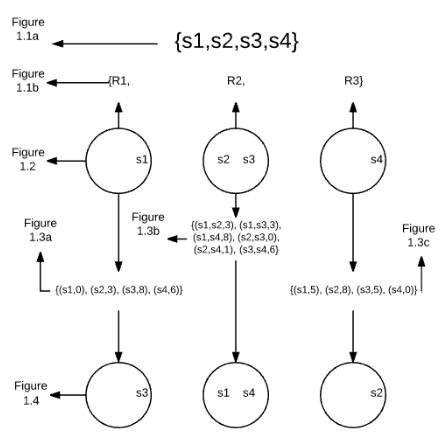
\includegraphics[scale=0.6]{model} 
\caption{Room Swap Model}
\end{figure}
%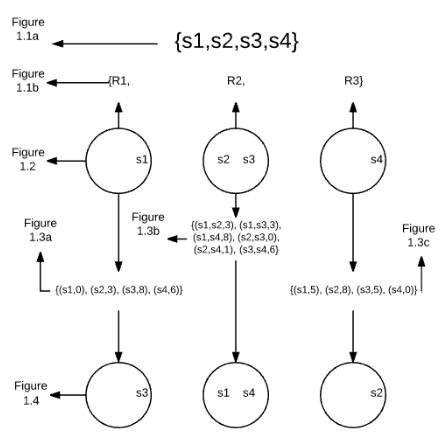
\includegraphics[scale=0.6]{model} %\qquad
\noindent As you can see in the above figure, room $r_1$ has one student in the swap, $s_1$, room $r_2$ has two students in the swap, $s_2$ and $s_3$, and room $r_3$ has one student in the swap, $s_4$. Figure 1.4 is the result of the optimal swap taking place, where student $s_3$ moves into $r_1$, students $s_2$ and $s_3$ move into $r_2$, and student $s_2$ moves into $r_3$. In Figures 1.3a-c each tuple consists of student(s) and a weight. The tuples containing the optimal swaps have the highest weight total of any other combination with 24.

\subsection{Preferences}
In the next section we will go into specifics about preferences we examined, preferences we picked, preferences that could be considered in future iterations of this project, and how we go about converting preferences into weights. In this section, our focus is to explain how preferences fit into the overall solution.\\

\noindent Preferences are what result in the weights in the model – they take into account two things; the personality compatibility of the roommates and the room characteristics. Students will fill out a form/survey and their answers will be compared to other students’ answers to try to predict compatibility. 

\subsection{Deal-breakers} 
Closely related to preferences is the concept of deal-breakers. The idea is that students can pick certain characteristics about a roommate that they deep unacceptable in a roommate. The application of deal-breakers is endless - one could choose to give every question the option of a deal-breaker. This is an approach we do not recommend because it would greatly reduce the number of feasible swaps. 
% Allowing each question to be a deal-breaker is an approach we do not recommend because it would greatly reduce the number of feasible swaps. 
\paragraph{Example.}
An example of how a deal-breaker could be applied to a preference is with the following question: \textit{Are you a smoker?} A person who doesn't smoke may not want to ever be placed in a room with someone that smokes cigarettes. We will walk through this example in more detail in the following section.

\section{Preferences}
%Now we'll discuss more in depth how we...
%Based on our model, We use edge weights to capture student preferences. 
In this section, we'll discuss in depth how we determined what preferences to consider , and how we calculated edge weights. 


\subsection{Specific Preferences Considered}
First, we came up with an initial list of important factors that could potentially affect students' overall satisfaction (level) of their room. The factors we deemed important included: 
\begin{itemize}[noitemsep]

\item Type of housing (Single Gender, Mixed gender, Gender Inclusive)
\item Whether the student smokes
\item Sexual Orientation
\item Major 
\item Age
\item Religion
\item Desired Location
\item Cleanliness
\item Significant Other
\item Going out frequency (nights/week)
\item Usual sleep/waking up time
\item Preferred place for studying
\end{itemize}
After coming up with this list, we realized some of some of these questions would be inappropriate to ask, and we were unsure if we would be allowed to ask them. For two questions specifically, we felt they might give us a good idea on how accepting of diversity students would be. For example, we thought religion might be important to some students. Additionally, we thought sexual orientation might be important to ask about. Ideally, the room swap does not place people in rooms where they are bound to be disliked right off the bat. Ultimately, we had to consider what we could ask according to university policy and decided to air on the side of caution with respect to these two questions. \\

\noindent We narrowed down the list to:
\begin{itemize}[noitemsep]
\item Smoking habits
\item Major 
\item Age
\item Desired Location
\item Cleanliness
\item Going out frequency (nights/week)
\item Usual sleep/waking up time
\item Preferred place for studying
\end{itemize}
\paragraph{Improvements.}
Students are required to provide information when applying for on-campus housing. Since typically, using the information for the student staying in the room. It didn't seem reasonable to require students staying in the room to fill out a form because their roommate was participating in the room exchange. This would also be inefficient because the roommate staying in the room would have to fill out the form multiple times in the case that subsequent roommates participated in the exchange, but their answers would probably be the same. Since ResLife requires students to provide basic information when applying for housing, we would (theoretically) just retrieve the information from there. Since some of this information is subject to change, a student could update their profile. 


\subsection{Calculating Weights}
%Trouble with calculating weights for binary preferences (smoking vs. nonsmoking) vs. living locations
We use edge weights to capture student preferences.
Based on our model, our edge weights represent the compatibility of a student to another student and the room. So we needed a way of converting their preferences, (that is, their responses to our questions), into a numeric value. 
This proved to be challenging because the format of their responses varied by question. Based on the nature of the answers to some of these questions we needed to come up with a method of converting these answers to a 'value'. For some of their responses, assigning a value was simple.
%Note that a room coul
\paragraph{Example.}
For example, converting age into a numeric value is simple. We would just subtract the difference of each students' age from some constant, $k$, where $k$ represents the maximum value weight we have determined this question should have. Below is code that would do that for us.

\lstinputlisting[language=Java, caption={Calculating Weight with Student Age}]{weightCalc.java}
\paragraph{Example.}
On the other hand, other preferences are far more challenging to assign a value, simply because responses to certain questions are far from just a number. Consider a case where we are trying to calculate a weight based on location. How would we measure the strength of a room assignment consisting of a student wanting to live in Leonardtown, but being evaluated for room located in Commons? Below is code that would do that for us.
%Supposed we had a student who selected 
\lstinputlisting[language=Java, caption={Calculating Weight with Location}]{locationCalc.java}
%\end{multicols}
In the above scenario, both Leanardtown and Commons are located on South Campus, so a value of one would be returned. Appropriately, this would be better than if the same student was being evaluated for a room on North Campus, while being worse than if the room was located in Leonardtown. 
\paragraph{Example.}
Earlier, we introduced the concept of deal breakers. There are a variety of ways to implement this and some approaches, possibly the best approaches, involve the use of an 'Answer' object that could have a deal breaker field. For the sake of simplicity, we will omit that in this example.
\lstinputlisting[language=Java, caption={Calculating Weight with Deal Breaker}]{smokerCalc.java}
In order to calculate the overall weight, or in other words, calculate the optimality of a room assignment for a student, one need only to add the sum of all of these weight calculating functions for each question in the form. To account for deal breakers, just look out for a negative weight at any time. These functions can be implemented in Java by using lambda functions, which could allow you to store weight calculations within a 'Question' object by invoking the constructor. Alternatively, you could choose to implement separate functions and just call them accordingly when going through this process.

\subsection{Other preferences to be considered}
There are a plethora of preferences you can consider when implementing a roommate swap. A few more ideas are:
\begin{itemize}[noitemsep]
\item AC in rooms
\item Ok with living in triples/doubles 
\item Prefer apartment setting
\end{itemize}

%\end{multicols} 
\section{Model}

\subsection{Some Kind of Graph?}
%Our general idea for the solution: graph structure; rooms are vertices, edges between vertices.
The data structure we determined would best fulfill our needs (requirements/conditions) was a graph. Each node in the graph represents a room, $r$. Each room has a capacity, $c_r$. Each edge has a weight, which represents the compatibility between the room/current resident, based on the preferences of the students. We decided to use Java, and have the following classes: Profile, Person, Question, Answer.
\paragraph{Person} The Person class would hold information about the person, such as the student's name, age, sex, major, contact information, the dorm he or she is currently living in.
\paragraph{Question}
The Question class would hold information about the question, the question, and a calculate weight method. The calculate weight method would have two Answer objects as parameters (arguments). Based on each student's answer, we would return a value. We realized depending on the question, the format of the answer, this would be hard to implement using generics. Coming up with a good design was challenging. We discuss this more in depth in the following section. 
%Lambda Expressions

\paragraph{Answer} The Answer class would hold a students answer to a question. If the Question had the option of being a 'deal-breaker', we would store this information as a boolean here as well.
\paragraph{Profile} The Profile class would hold all the answers to the questions.  

\subsection{Lambda Expressions}
%Should we talk about this?\\
%The problem. 
%How lambda calculus solves the problem.
At first we had difficulty coming up with a efficient design that allowed us to include different weight functions between ``Questions". Since the calculate weight method of the Question class determined the weight, we needed to include the functionality of this method as an argument. We eventually found a solution using Java Lambda expressions. Java Lambda expressions allows us to include our function as an argument. Using the BiFunction Interface, we can take answers from two students and translate their responses into numerical value, regardless of the nature or format of their responses. 

\paragraph{BiFunction Interface}
The BiFunction Interface represents a function that accepts two arguments and produces a result. In our case the two arguments are student responses, and the result will be a numerical value-- specifically, an integer. 

\paragraph{Examples}
For example, consider our age response again. The weight function for students' ages would be implemented as follows.

\lstinputlisting[language=Java, caption={Calculating Weight with Student Age}]{lambda_example.java}
Assigning a weight is simple, however. On the other handle, responses are a little more tricky. For example, consider location. 
%Supposed we had a student who selected 
\lstinputlisting[language=Java, caption={Calculating Weight with Location}]{location_example.java}
%\end{multicols}

\section{Optimization Algorithm}

Up until now we've thought of our rooms as nodes in a graph. Now we'll look at the data as sets of potential occupants of the room. First, some terminology:\\

\noindent{Rooms $\cal R$; \qquad with each $r\in{\cal R}$\qquad with capacity $c_r\in\mathbb{Z^+}$}\\
\noindent{Students $\cal S$; \qquad with each $s\in{\cal S}$}\\ 

\noindent We're going to be doing most of our optimizing on variable x:

\begin{equation*}
\noindent{x_r^s \in \{0, 1\}\\} 
\end{equation*}

\noindent{$s$ is student set \#\\
$r$ is old room \#}

\noindent{0 if they don't go to room, 1 if they do. }\\

What we're going to be maximizing, since this is an optimization problem, is W(R,S). As you recall each edge has a weight w(r,s), and W is the sum of all of the weights from each student wherever they end up. So our optimization equation is:\\

\begin{equation*}
\max\sum_{r\in{R}}\sum_{s\in{S(r)}}w(r,s)\cdot{x_s^r}\quad{s.t.}\\
\end{equation*}

With the constraints that each student gets assigned to a room and makes sure each only gets assigned to one room.

\begin{align*}
\forall{s}&\in{S}\sum_{r\in{R}}\sum_{s\in{S(r)}}x_s^r=1\\
\forall{r}&\in{R}\sum_{s\in{S(r)}}x_s^r=1
\end{align*}

Let's take a look at an example:\\

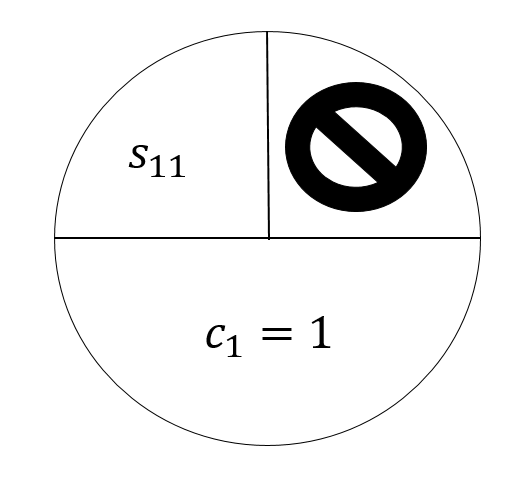
\includegraphics[scale=0.25]{c1} %\qquad \qquad
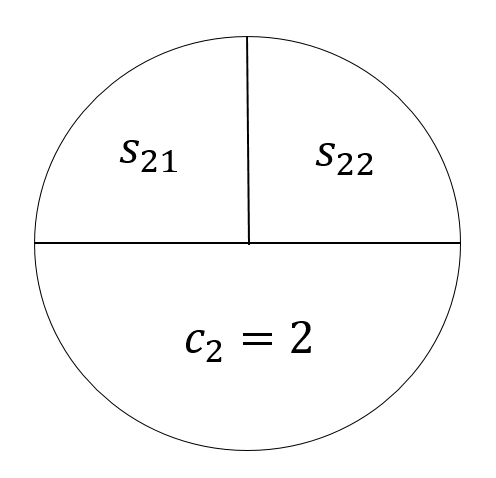
\includegraphics[scale=0.25]{c2} %\qquad \qquad
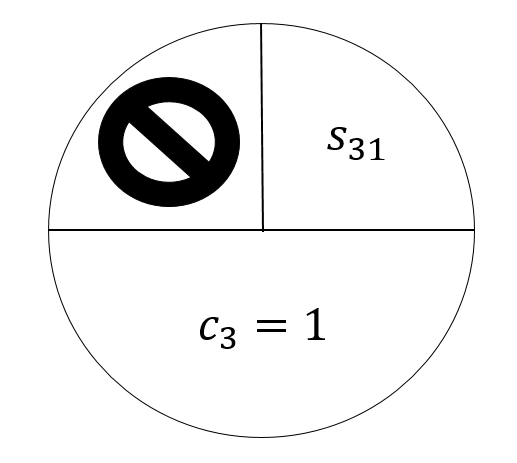
\includegraphics[scale=0.25]{c3}

\includegraphics[scale=0.5]{symbol}
(Occupied room)\\

Each node $r\in{\cal R}$, has a set of potential sets that could move into that node. If there is one vacancy in the room, it will be sets of one which we will just denote as singular objects for convenience. However, in the case of node $r_2$ above, the set will be sets of two.

\begin{align*}
r_1&= \{s_{11}, s_{21}, s_{22},s_{31}\}\\
r_2&= \{\{s_{11}, s_{21}\}, \{s_{11},s_{22}\},\{s_{11},s_{31}\},  \{s_{21},s_{22}\}, \{s_{21},s_{31}\},  \{s_{22},s_{31}\} \}\\
r_3&= \{s_{11}, s_{21}, s_{22},s_{31}\}\\
\implies x_r^s \in \{0, 1\}
\end{align*}

%\begin{equation*}
%r_1 = \{s_{11}, s_{21}, s_{22},s_{31}\}\\
%r_2 = \{\{s_{11}, s_{21}\}, \{s_{11},s_{22}\},\{s_{11},s_{31}\},  \{s_{21},s_{22}\}, \{s_{21},s_{31}\},  \{s_{22},s_{31}\} \}\\
%r_3 = \{s_{11}, s_{21}, s_{22},s_{31}\}\\
%\implies x_r^s \in \{0, 1\}
%\end{equation*}

\begin{align*}
x_2^1+x_1^2+x_4^2&=1\\
x_5^2+x_2^3&=1\\
\end{align*}

%\begin{multicols}{2}

\section{Integer Programming}
In order to determine how to optimize our swapping, Dr. Dickerson introduced us to integer programming. He has used it previously to solve similar problems with swapping markets. Most of the knowledge (with the addition of some wikipedia) we learned about integer programming came from Dr. Dickerson and also a lecture off of MIT's OpenCourseWare (citation?).
% \cite{orlin}

\subsection{So what is integer programming?}
Integer programming solves combinatorial optimization problems. Each room has $s$ (\# students) choose $c_r$ (capacity of the room) possibilities for who can stay in there. The structure of a problem that can be solved. 

\subsection{Why will this work?}
So as we've just described, integer programming optimizes (by minimizing or maximizing) a value. In our case, integer programming maximizes the sum of the weights of people swapping rooms. That is our main goal and it is fulfilled by this algorithm. Also, since we've imposed our constraints on the system (each student gets put in one room and only one room), we know that the result outputted will be a feasible solution. Therefore we know the solution outputted will be an implementable solution, but that leaves for all kinds of potential corner cases. One example is if the optimal solution is that everybody stays where they are. This is highly unlikely because it would mean that all weights are zero. A more likely case is that the algorithm leaves some people where they are. This does not seem like it would optimize the system but if one person is extremely hard to deal with, leaving them where they are might be the best option. That person may have to relax their preferences and re-enter the swap to find a good roommate. Regardless of the results, we know this will work for us if we compose the appropriate inputs and write the constraints properly and then put it into a black box solver. As we've already described the algorithm it will output the happiest weighted set of assignments.

\section{Future Work- Data Analysis}
Initially we struggled to determine what we should do to show results for our algorithm. We were originally thinking we would want to compare the same inputs on our system as theirs and see which was better. However, we got no information from Reslife throughout the semester so using results in our analysis at all wasn't going to happen. We had to choose a new way to validate our work.

\subsection{Testing Speed of Algorithm}
Our first attempt to try and  we might just run our own algorithm on 10 students, then 100, then 10,000 to see how the speed decreases with runs. But, we realized that wasn't really a useful metric to rate our algorithm by because not that many students enter the room swap. UMD has 4,000 students living on campus so it doesn't really reach that volume.

\subsection{Surveys}
During our presentation in class Dr. Hicks suggested that we could survey people to find out how they feel about their room situation.

\section{Future Work- Room to Expand}
We didn't realize that we were spending too much time worrying about the preferences and as such didn't get to implement everything that we discussed. There are a couple topics we talked about how we would deal with but decided to cut them for the purposes of this class.\\
-multi-gender housing situations (we assumed everyone in the swap is of the same gender to eliminate this confusion)\\
-what else did we eliminate?

\section{Works Cited}
"Introduction to Integer Programming - Integer Programming Models." The Lancet (2013). http://ocw.mit.edu. MIT OpenSourceWare, 14 Mar. 2013. PDF.

%\end{multicols}
%\bibliographystyle{ieeetr}
%\bibliography{references} 

\end{document}